%\documentclass[a4paper,12pt]{article}
\documentclass[landscape,20pt,dvips]{foils}
%\usepackage{xspace,colortbl}     % should have txfonts also

\usepackage{fancyvrb}
%\usepackage{verbatim}
\usepackage{subfigure}
\RequirePackage{ifthen}
\RequirePackage{times}      % Loads the Times-Roman Fonts
\RequirePackage{mathptm}    % Loads the Times-Roman Math Fonts
\RequirePackage{pifont}     % Loads the Postscript symbol fonts
\usepackage{amssymb}

	\newif\ifpdf
	\ifx\pdfoutput\undefined
        \pdffalse
	\else
        \pdfoutput=1
        \pdftrue
    \fi
% Set up PDF specific
	\ifpdf
        %\renewcommand\url\undefined % sorry, tex2page, hyperref provides its own
        % use HyperRef for PDF hyperlinks etc
	    \usepackage[pdftex,colorlinks=true,urlcolor=blue,pdfstartview=FitH]{hyperref}
	    \pdfcompresslevel=9
        \hypersetup{
          pdftitle={From Python to PLT Scheme},
          pdfauthor={Daniel Silva and Philippe Meunier, Northeastern University},
          %pdfpagemode={FullScreen},
          pdfborder={0 0 0}
          }
        % PDF graphics
        \usepackage[pdftex]{graphicx}
		\DeclareGraphicsExtensions{.pdf}
        \usepackage[pdftex]{geometry}
        % use colors
        \usepackage[pdftex]{color}
	\else
        \usepackage{geometry}
        \usepackage{graphicx}
        \usepackage{url}
        \usepackage{color}
	\fi

% set the slide layout
%\geometry{headsep=1.0em,hscale=0.80}
\geometry{vscale=0.80,hscale=0.80}

% define new colors
\definecolor{vinho}{rgb}{0.6,0,0}
\definecolor{myblue}{rgb}{0,0.2,0.4}
% default color
\color{black}
% note: to set color for a block use {\textcolor{vinho} Hello World}

\usepackage{multicol}           % Multi-column formatting

\usepackage{foilspagecounting} % http://www-users.york.ac.uk/~zrs1/Software/pagecounting.html

\usepackage{listings} % typeset source code

% bring the body text a little closer
\newlength\oldfoilheadskip
\setlength\oldfoilheadskip{\foilheadskip}

\newcommand{\jhead}[1]{\foilhead{\flushleft \textcolor{vinho}{\large   #1}
\vspace{-0.84cm} \\ {\color{black} --------------------------------------------------------------- }}}


%\newcommand{\lastpage}[0]{woot}
%\AtEndDocument{\write\@auxout{\string\lastpage{\thepage}}}

%\def\lastpage{0}
%\AtEndDocument{%
%  \clearpage
%  \addtocounter{page}{-1}
%  \immediate\write\@auxout{\string\gdef\string\lastpage{\thepage}}}


% Other useful macros for doing slides.
%\newcommand{\red}[1]{{\color{red} #1}}
%\newcommand{\blue}[1]{{\color{blue} #1}}
%\newcommand{\black}[1]{{\color{black} #1}}

% The title of a slide
%\newcommand{\slideheading}[1]{
%  {\normalfont\LARGE\bfseries\sffamily\color{section2}#1}
%  \vspace*{0.1in}
%  }

%%%%%%%%%%%%%%%%%%%%%%%%%%%%%%%%%%%%%%%%%%%%%%%%%%%%%%%%%%%%%%%%%%%%%%%%%%%%%%%
%%%%%%%%%%%%%%%%%%%%%%%%%%%%%%%%%%%%%%%%%%%%%%%%%%%%%%%%%%%%%%%%%%%%%%%%%%%%%%%

\title{\emph{\color{vinho} From Python to PLT Scheme}}
\author{\color{black} Daniel Silva, Philippe Meunier \\
\texttt{\color{black} \small dsilva, meunier@ccs.neu.edu}}

\date{\today}

\rightfooter{\includegraphics[height=1cm]{figures/plt-logo}}

%-----------------------------------------------------------------------
%-----------------------------------------------------------------------
\begin{document}
\MyLogo{\hspace{-0.5cm} \color{black} \tiny College of Computer and Information Science : Northeastern University}

\maketitle

\vspace{1cm}
%\centerline{
\includegraphics{figures/PLTnolarval}}
\centerline{
\includegraphics{figures/plt}}

%----------------------------------------
\jhead{The Spy Project Motivation and Goals}
\MyLogo{}
\LogoOff

\begin{itemize}
  \item Motivation
  \begin{itemize}
    \item DrScheme is a good PDE with nice tools
    \item Python is popular (many users, many libraries)
    \item Python should map easily to Scheme
    \item We want DrScheme (with tools) + Python (with libraries)
  \end{itemize}
  \item Goals
  \begin{itemize}
    \item Support the Python language
    \item Support DrScheme tools
    \item Support the CPython FFI
  \end{itemize}
  \item Warnings
  \begin{itemize}
    \item Experimental project
  \end{itemize}
\end{itemize}

%----------------------------------------
\jhead{Overview}

\begin{itemize}
  \item Spy Structure
  \item Translations (and Problems)
    \begin{itemize}
      \item Functions
      \item Classes
      \item Modules
    \end{itemize}
  \item Status
    \begin{itemize}
      \item Language
      \item C Extensions
      \item Performance
      \item DrScheme Tools
    \end{itemize}
  \item Future Work
\end{itemize}

%----------------------------------------
\jhead{Assumptions}
  \begin{itemize}
    \item MzScheme
    \begin{itemize}
       \item First-class, dynamic namespaces
       \item Hash tables
    \end {itemize}
    \item Python
    \begin{itemize}
       \item First-class, dynamic modules
       \item Dictionaries
    \end {itemize}
  \end{itemize}

%----------------------------------------
\setlength\foilheadskip{-1cm}
\jhead{Spy Structure}
\setlength\foilheadskip{\oldfoilheadskip}

\begin{center}
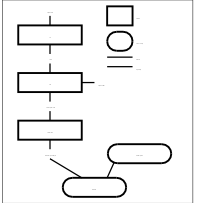
\includegraphics[height=15.65cm]{figures/compiler-overview-compressed}
\end{center}

%----------------------------------------
\jhead{Translations: Functions}
\lstset{language=Python}
\begin{lstlisting}
def f(pos, def_arg = 1, *rest, **kw_args):
  return 1
\end{lstlisting}

  \begin{itemize}
    \item defined by putting the name in the right namespace
    \item default arguments in \emph{opt-lambda}
    \item Python rest args mapped to Scheme rest args
    \item Python keyword args passed as first argument
    \item \emph{return} statements implemented with escape continuations
  \end{itemize}
%----------------------------------------
\jhead{Translations: Classes: Problems}
\begin{lstlisting}
class C:
  def meth(this, x):
    return this.y + x
\end{lstlisting}
  \begin{itemize}
    \item Python OO system is completely dynamic
      \begin{itemize}
        \item Objects are hash tables
        \item Attribute access (\verb|obj.attr|) is sugar (\verb|obj.__dict__['attr']|)
        \item Mutable internal hash table accessed via \verb|obj.__dict__|
        \item Classes are mutable objects
      \end{itemize}
    \item MzScheme classes are immutable
    \item Mixins create new classes
    \item Multiple inheritance in Python vs. single in MzScheme
  \end{itemize}
%----------------------------------------
\jhead{Translations: Classes: Solution}
    Spy emulates Python objects
\\
\lstset{language=Lisp, morekeywords={lambda, opt-lambda}, emph={rest}}
\begin{lstlisting}
; a PyObject is a:
; (make-python-node PyObject hash-table boolean)
(define-struct python-node (type dict mutable?))

(define C
 (make-python-node type
                   (assoc-list->hash-table
                     `((__bases__ ,(->py (list object)))
                       (__name__ ,(->py "C"))
                       (meth ,(->py (lambda (this x)
                                               ...)))))
                   #t))
\end{lstlisting}
%----------------------------------------
\jhead{Translations: Modules}
\lstset{language=Python}
\begin{lstlisting}
if I_feel_like_importing_you:
  import something from you
  something()
else:
  import m
  m.some_parameter = "overridden"
\end{lstlisting}
  \begin{itemize}
    \item MzScheme modules incompatible
      \begin{itemize}
        \item No cycles
        \item No assignments across modules
      \end{itemize}
    \item Namespaces support assignment (\verb|namespace-set-variable-value!|)
    \item $\therefore{}$ Python modules translated using MzScheme namespaces
  \end{itemize}
%----------------------------------------
\jhead{Status: Language}
  \begin{itemize}
    \item Most of Python implemented
    \item To do:
    \begin{itemize}
      \item \emph{yield}
      \item \emph{exec}
      \item extended slices
    \end{itemize}
  \end{itemize}
%----------------------------------------
\setlength\foilheadskip{-1cm}
\jhead{Status: Language Example: Classes}
\setlength\foilheadskip{\oldfoilheadskip}

\begin{center}
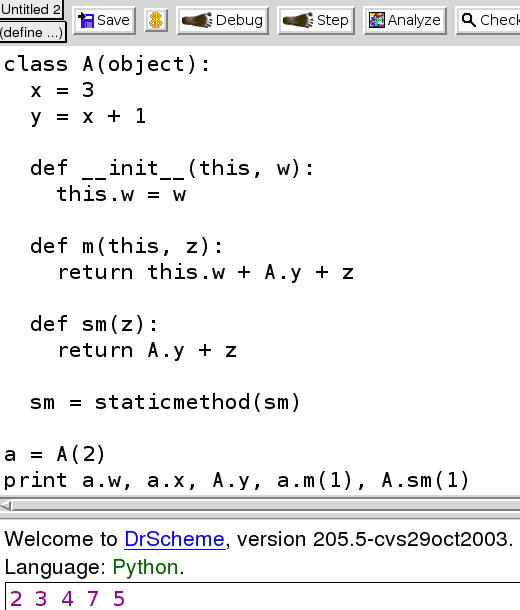
\includegraphics[height=15.65cm]{figures/spy-class-with-staticmethod-oct-30-2003}
\end{center}
%----------------------------------------
\jhead{Status: Runtime Library}
  \begin{itemize}
    \item Too much boring work to re-implement
      \begin{itemize}
        \item addition
        \item subtraction
        \item \emph{append}
        \item \emph{string-append}
        \item etc\ldots
      \end{itemize}
    \item Strategy: use CPython's standard modules
  \end{itemize}
%----------------------------------------
\jhead{Status: C Extensions}
  \begin{itemize}
    \item Experimental support
    \item CPython's \verb|stringobject.c| loads correctly
    \item Still work to do on a simple tool:
    \begin{itemize}
      \item \verb|mzc --spy pyGtk.c|
    \end{itemize}
  \end{itemize}
%----------------------------------------
\jhead{Status: Performance}
  \begin{itemize}
    \item Horrible (3 orders of magnitude slower)
    \item Too many indirections
    \item Very inefficient runtime library
  \end{itemize}
%----------------------------------------
\setlength\foilheadskip{-1cm}
\jhead{Status: DrScheme Tools: Check (well-formed) Syntax}
\setlength\foilheadskip{\oldfoilheadskip}

\begin{center}
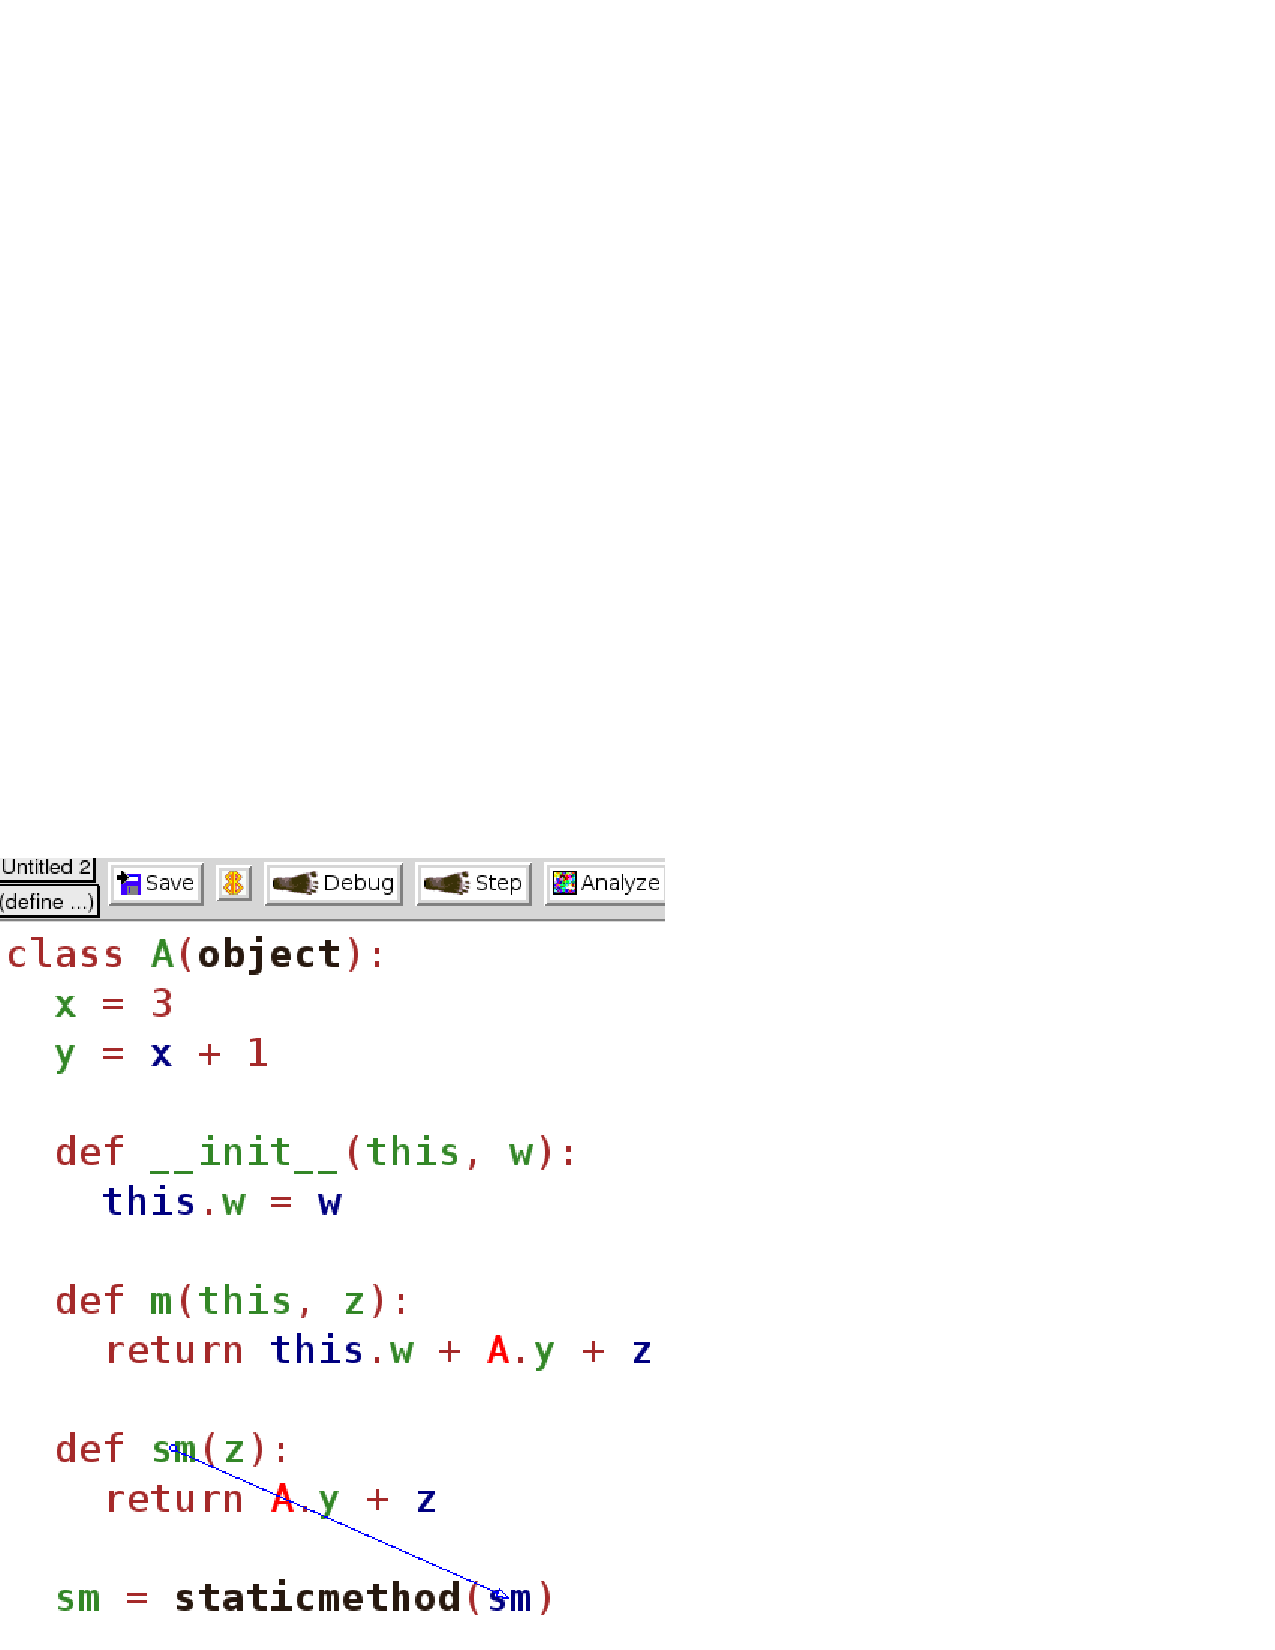
\includegraphics[height=15.65cm]{figures/spy-check-syntax-oct-30-2003}
\end{center}

%----------------------------------------
\setlength\foilheadskip{-1cm}
\jhead{Status: DrScheme Tools: Test Coverage}
\setlength\foilheadskip{\oldfoilheadskip}

\begin{center}
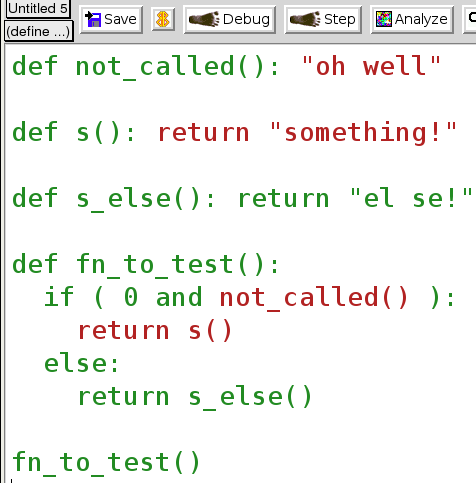
\includegraphics[height=15.65cm]{figures/spy-expression-test-coverage-oct-30-2003}
\end{center}
%----------------------------------------
\jhead{Status: DrScheme Tools: Incompatibilities}
  \begin{itemize}
     \item MrFlow
     \begin{itemize}
        \item No type-based flow information for primitives yet.
     \end{itemize}
     \item Stepper
     \begin{itemize}
        \item No decompiler yet.
     \end{itemize}
     \item Debugger
     \begin{itemize}
        \item Spy can be instrumented to work with the debugger.
        \item Not done yet though.
     \end{itemize}
  \end{itemize}
%----------------------------------------
\jhead{Future Work}
  \begin{itemize}
     \item Comprehensive Python language support
     \item Full C extension compatibility
     \item Simple Python $\longleftrightarrow$ Scheme interoperability
\lstset{language=Lisp, morekeywords={lambda, opt-lambda}, emph={rest}}
\begin{lstlisting}
(py-eval "x = 1")
(in-python (ns-set! 'x
                    (->py (+ 2
                             (->scheme (ns-get 'x))))))
(py-eval "print x") ; 3
\end{lstlisting}
  \end{itemize}
%----------------------------------------
\jhead{Conclusion}
  \begin{itemize}
     \item Spy interprets most of Python
     \item Spy brings DrScheme \& tools to Pythonistas
     \item Spy brings Python libraries to Schemers
     \item Spy loves volunteers --- contact us.
     \begin{itemize}
        \item e-mail: \url{dsilva@ccs.neu.edu}
        \item website: \url{http://spyweb.hopto.org}
     \end{itemize}
  \end{itemize}
%----------------------------------------
\jhead{Thanks}
  We thank Matthias Felleisen for his guidance.

  Thanks to Scott Owens for developing the Spy lexer and parser.

%----------------------------------------
\jhead{PLT Spy}

\vspace{4cm}

\begin{center}
Questions?
\end{center}

\end{document}
